\documentclass[10pt,twocolumn, nofootinbib]{revtex4-2}
%\documentclass[aps,pra,10pt,twocolumn,floatfix,nofootinbib]{revtex4-1}
%\documentclass[10pt,twocolumn,letterpaper]{article}

\usepackage{amsmath}
\usepackage{amssymb}
\usepackage{graphicx}
\usepackage{amsfonts}
\usepackage{enumitem}
\usepackage{graphicx}
\usepackage{hyperref}
\usepackage{tikz}

\hypersetup{
	colorlinks=true,
	citecolor=blue,
	urlcolor=blue,
	linkcolor=blue
}
\urlstyle{same}
\frenchspacing

\newcommand\partitle[1]{\textsc{#1}.}


\begin{document}

\title{A no-go theorem for $\psi$-ontic models}
\author{Gabriele Carcassi}
\affiliation{Physics Department, University of Michigan, Ann Arbor, MI 48109}
\author{Andrea Oldofredi}
\affiliation{Centre of Philosophy, University of Lisbon, Portugal}
\author{Christine A. Aidala}
\affiliation{Physics Department, University of Michigan, Ann Arbor, MI 48109}

\date{}


\begin{abstract}
In this note we give a simple argument as to why $\psi$-ontic models cannot be expected to reproduce quantum mechanics. We will see that, using information theoretic considerations, the lack of overlap of epistemic states requires all states to be orthogonal, which directly contradicts quantum theory. This argument is a much simplified version of the one we presented in a previous paper.
\end{abstract}

\maketitle

\section{Introduction}


\section{The argument}

What we want to show is that a set of non-overlapping probability distributions cannot reproduce the entropy given by quantum mechanics. Let us review a couple of properties of the information entropy, both in the classical setting (i.e. the Shannon/Gibbs entropy) and in the quantum setting (i.e. the von Neumann entropy).\footnote{We leave the calculations in the appendix.}

\textbf{Entropy of mixed non-overlapping distributions}. Let $\rho_1$ and $\rho_2$ be two classical distributions over a space $\Lambda$ with measure $\lambda$. The entropy will be given by\footnote{The logarithm is assumed to be in base 2.}
\begin{equation}\label{shannon_entropy}
	H(\rho_1) = - \int_\Lambda \rho_1(\lambda) \log \rho_1(\lambda) d\lambda.
\end{equation}
Suppose the two distributions are disjoint, and let $\rho = \frac{1}{2} \rho_1 + \frac{1}{2} \rho_2$ be a uniform mixture of the two distributions. The entropy of $\rho$ is given by
\begin{equation}\label{entropy_nonoverlap}
	H(\rho) = 1 + \frac{1}{2} H(\rho_1) + \frac{1}{2} H(\rho_2).
\end{equation}
Note how the non-overlapping assumption fixes the entropy of the mixed state.

\textbf{Entropy of quantum mixed states}. Now suppose $\psi$ and $\phi$ are two pure quantum states and let $p = | \langle \psi | \phi \rangle |^2$ be the probability of transition from one to the other. Consider the mixed state $\rho = \frac{1}{2} | \psi \rangle \langle \psi | + \frac{1}{2} | \phi \rangle \langle \phi |$. Its entropy is given by
\begin{equation}\label{entropy_mixed}
	H(\rho) = H\left(\frac{1+\sqrt{p}}{2}, \frac{1-\sqrt{p}}{2}\right).
\end{equation}

\textbf{Non-overlapping distributions can only represent orthogonal states}. Now, suppose we have a $\psi$-ontic model. The epistemic states $p(\lambda|P_\psi)$ and $p(\lambda|P_\phi)$ consist of non-overlapping distributions over a space $\Lambda$, therefore eq. \ref{entropy_nonoverlap} applies. Given that $\psi$ and $\phi$ are pure states, and the entropy for pure states is zero, we must have
\begin{equation}\label{entropy_pure}
	H(p(\lambda|P_\psi)) = H(p(\lambda|P_\phi)) = 0,
\end{equation}
and therefore
\begin{equation}\label{required_entropy}
	\begin{aligned}
	H\left(p(\lambda|\frac{1}{2}P_\psi + \frac{1}{2}P_\phi)\right) &= \\
H\left(\frac{1}{2}p(\lambda|P_\psi) + \frac{1}{2}p(\lambda|P_\phi)\right) 
&= 1.
	\end{aligned}
\end{equation}
If we compare the above with eq. \ref{entropy_mixed}, it follows that $p$ must be zero. That is, we must have that
\begin{equation}\label{orthogonal}
	 \langle \psi | \phi \rangle = 0
\end{equation}
no matter what $\psi$ and $\phi$ are.

The non-overlapping assumption built into the $\psi$-ontic model necessarily implies that all pure states are orthogonal. Since this is not true in quantum mechanics, any $\psi$-ontic models will fail to reproduce the results of quantum information, quantum statistical mechanics and, therefore, quantum theory in general.

In retrospect this should not be surprising for two reasons. First of all, the case where all states are orthogonal is exactly the case for which all observables commute, the classical case. Therefore we are simply finding that the implicit use of classical probability in $\psi$-ontic models pushes us to the classical case. Secondly, we already know that quantum information theory has features that are not reproducible in classical information theory, and that is exactly what makes it such an exciting new field.


\section{Conclusion}

We have presented a much simpler version of the argument presented in [cite] to reach the same conclusion: $\psi$-ontic models are not compatible with quantum information theory and therefore quantum theory itself. The finding is consistent with our claim that the ontological model has a hidden assumption of non-contextuality (through the use of standard Kolmogorov probability), which here can be seen to force all pure states to be orthogonal, to belong to the same context, as they do in classical mechanics.

One may think the problem could be circumvented by substituting the Shannon entropy formula. That is, the problem is not with the non-overlapping assumption but rather with how the entropy is calculated. However, the link between probability theory, information theory and measure theory is so tight that it makes this approach unfeasible: failure of one means failure of all. We will look deeper into this issue in a later work.

\section*{Appendix: calculation}

\textbf{Entropy of mixed non-overlapping distributions}. We want to show that, given two non-overlapping probability distributions $\rho_1$ and $\rho_2$, the entropy of $\rho = \frac{1}{2} \rho_1 + \frac{1}{2} \rho_2$ is given by
\begin{equation}\label{entropy_nonoverlap_appendix}
	H(\rho) = 1 + \frac{1}{2} H(\rho_1) + \frac{1}{2} H(\rho_2).
\end{equation}

Let $U_1, U_2 \subset \Lambda$ be the respective supports of the distributions. Since the distributions are non-overlapping, we have $U_1 \cap U_2 = \emptyset$. We have
\begin{align*}
	H(\rho) &= - \int_\Lambda \rho \log \rho d\lambda \\
	&= -\int_{U_1} \rho \log \rho d\lambda -\int_{U_2} \rho \log \rho d\lambda \\
	&= -\int_{U_1} \frac{1}{2} \rho_1 \log \frac{1}{2} \rho_1 d\lambda -\int_{U_2} \frac{1}{2} \rho_2 \log \frac{1}{2} \rho_2 d\lambda \\
	&= - \frac{1}{2} \int_{U_1} \rho_1 \log \frac{1}{2} d\lambda - \frac{1}{2} \int_{U_1} \rho_1 \log \rho_1 d\lambda \\
	&- \frac{1}{2} \int_{U_2} \rho_2 \log \frac{1}{2} d\lambda - \frac{1}{2} \int_{U_2} \rho_2 \log \rho_2 d\lambda \\
	&= - \frac{1}{2} \log \frac{1}{2} - \frac{1}{2} \log \frac{1}{2} + \frac{1}{2} H(\rho_1) + \frac{1}{2} H(\rho_2) \\
	&= 1 + \frac{1}{2} H(\rho_1) + \frac{1}{2} H(\rho_2) \\
\end{align*}


\textbf{Entropy of quantum mixed states}. We want to show that, given two states $\psi$ and $\phi$, the entropy of the mixed state $\rho = \frac{1}{2}|\psi\rangle\langle\psi| + \frac{1}{2}|\phi\rangle\langle\phi|$ is
\begin{equation}\label{entropy}
	H(\rho) = H\left(\frac{1+|\langle\psi|\phi\rangle|}{2}, \frac{1-|\langle\psi|\phi\rangle|}{2}\right).
\end{equation}

\begin{center}
	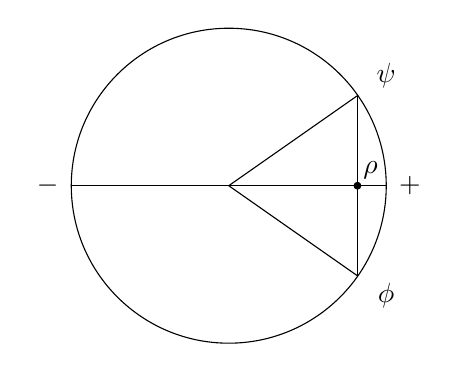
\begin{tikzpicture}[scale = 1]
		\draw (0,0) circle (2);
		\node at (-2.3,0) {$-$};
		\node at (2.3,0) {$+$};
		\node at (2,1.4) {$\psi$};
		\node at (2,-1.4) {$\phi$};
		\draw (-2,0) -- (2,0);
		\begin{scope}
			\clip(0,0) circle (2);
			\draw (0,0) -- (2,1.4);
			\draw (0,0) -- (2,-1.4);
			\draw (1.634,1.4) -- (1.634,-1.4);
		\end{scope}
		\fill (1.634,0) circle (0.05);
		\node at (1.8,.2) {$\rho$};
	\end{tikzpicture}
\end{center}

Note that $\psi$ and $\phi$ will identify a two-dimensional subspace which can be thought, without loss of generality, as a qubit and therefore can be represented by a Bloch sphere. The picture represents the intersection of the Bloch sphere with the plane identified by $\psi$ and $\phi$. As $\rho$ is an equal mixture of the two states, it will be represent by the midpoint between the two. Taking the line that goes through $\rho$ and the center of the sphere, we can see that $\rho$ can also be seen as the mixture of the states $+$ and $-$ which, since they represent equal and opposite directions, form a basis. To diagonalize $\rho$, then, means to express it in terms of $+$ and $-$.

If $\theta_{\psi\phi}$ is the angle between $\psi$ and $\phi$, we have
\begin{equation}
	|\langle \psi | \phi \rangle |^2 = \cos^2 \frac{\theta_{\psi\phi}}{2}.
\end{equation}
The angle is divided by two because the angle on the Bloch sphere (i.e. in physical space) is double the angle in the Hilbert space. For example, for $z^+$ and $z^-$ the angle on the Bloch sphere would be $\pi$ and the inner product is zero (i.e. opposite directions in physical space correspond to orthogonal states).

Now we express $\psi$ and $\phi$ in terms of $+$ and $-$, remembering that they form a basis. Given that $\rho$ is at the midpoint, the figure is vertically symmetric. The angle between $\psi$ and $+$, then, is half of $\theta_{\psi\phi}$. The inner product between $\psi$ and $+$ is
\begin{equation}
	\begin{aligned}
	|\langle \psi | + \rangle |^2 &= \cos^2 \frac{\theta_{\psi +}}{2} \\
&= \cos^2 \frac{\theta_{\psi\phi}}{4}.
	\end{aligned}
\end{equation}
Keeping in mind that we are composing vectors in the Hilbert space (and not in the geometry of the physical space) we have
\begin{align*}
	\left|\psi\right>&=\cos\frac{\theta_{\psi\phi}}{4}\left|+\right>+\sin\frac{\theta_{\psi\phi}}{4}\left|-\right> \\
	\left|\phi\right>&=\cos\frac{\theta_{\psi\phi}}{4}\left|+\right>-\sin\frac{\theta_{\psi\phi}}{4}\left|-\right>.
\end{align*}

The density matrices corresponding to the pure states are
\begin{align*}
	\left|\psi\right>\left<\psi\right|&=\cos^2\frac{\theta_{\psi\phi}}{4}\left|+\right>\left<+\right|\\
	&+\cos\frac{\theta_{\psi\phi}}{4}\sin\frac{\theta_{\psi\phi}}{4}\left(\left|+\right>\left<-\right|+\left|-\right>\left<+\right|\right) \\
	&+\sin^2\frac{\theta_{\psi\phi}}{4}\left|-\right>\left<-\right| \\
	\left|\phi\right>\left<\phi\right|&=\cos^2\frac{\theta_{\psi\phi}}{4}\left|+\right>\left<+\right|\\
	&-\cos\frac{\theta_{\psi\phi}}{4}\sin\frac{\theta_{\psi\phi}}{4}\left(\left|+\right>\left<-\right|+\left|-\right>\left<+\right|\right) \\
	&+\sin^2\frac{\theta_{\psi\phi}}{4}\left|-\right>\left<-\right|.
\end{align*}

We can now calculate the mixture
\begin{align*}
	\frac{1}{2}(|\psi\rangle\langle\psi| &+ |\phi\rangle\langle\phi|) \\
	&=\cos^2\frac{\theta_{\psi\phi}}{4}\left|+\right>\left<+\right| +\sin^2\frac{\theta_{\psi\phi}}{4}\left|-\right>\left<-\right| \\
	&=\frac{1+\cos\frac{\theta_{\psi\phi}}{2}}{2}\left|+\right>\left<+\right| +\frac{1-\cos\frac{\theta_{\psi\phi}}{2}}{2}\left|-\right>\left<-\right| \\
	&=\frac{1+|\langle\psi|\phi\rangle|}{2}\left|+\right>\left<+\right| +\frac{1-|\langle\psi|\phi\rangle|}{2}\left|-\right>\left<-\right|. \\
\end{align*}

As $\rho$ is in a diagonal form, the entropy is given by eq.~\ref{entropy}.


\bibliography{bibliography}


\end{document}